%%% 関西大学 総合情報学部 松下ゼミ 進捗報告 TeXテンプレート Ver 1.1 (2011/12/04) %%%
\documentclass{matsushita-zemi}
\usepackage[dvipdfmx]{graphicx}
\graphicspath{{./fig/}}

%%% タイトル (長くなる場合は¥¥で適宜改行すること)%%%
\title{HogeHogeにおけるHogeに関する研究}

%%% 氏名 (姓・名の間は半角スペース) %%%
\author{内藤 峻}

\begin{document}
\maketitle


%%% 以下、本文 %%%
\section{はじめに}
\label{background} 
近年、様々な情報が電子化されネットワーク上に蓄積されている。それに伴いこれらの情報を利用して、意思決定や問題解決に役立てる試みがなされている。しかし、情報は情報洪水と言われるほど増加しており現在の検索技術、言うなれば「情報の在処を見つける」ものではユーザの要求に十分に答えることができない。そこで、私はこのようなユーザの要求に応えるために「情報を理解する」検索技術を提案する。

\section{先行研究}
\label{relatedworks} 


\section{卒論にむけて}
\subsection{本研究の着眼点}

\subsection{研究進捗状況}
現在、図\ref{LTCond} ならびに図\ref{LCDCond} に示すような二つの実験環
境を作成し、表\ref{exp} に示す 4 群を対象に、被験者間実験をデザインし
ている。実験課題には、迷路上で 1 名の逃亡者を 3 名の追跡者が追いかけて
捕まえるタイプの課題(迷路課題)を用いる。現在、本課題のプログラムを 
Processing で作成しており、クライアント部が完成、サーバ部も 8 割の実装
が完了している。8 月末までにサーバ部を実装し、テストトライアルを行うと
ともに、その結果を反映させた改良を行う。その後、ゼミ外から被験者 80 名
を募集し、本実験を行う。本実験は9月から10月を予定している。

%% 図の挿入 (captionが下)
\begin{figure}[b]
 \centering
 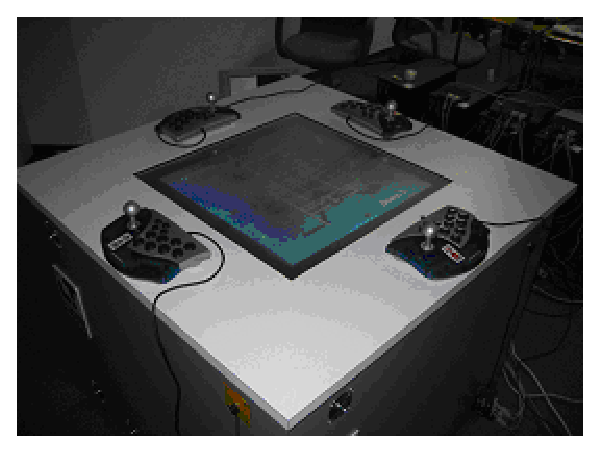
\includegraphics[width=0.4\columnwidth]{LTCond.eps}
 \caption{Lumisight Table 条件}
 \label{LTCond}
\end{figure}

%% 表作成 (captionが上)
\begin{table}[p]
\caption{実験群}
\label{exp}
\begin{center}
\begin{tabular}{lcc}
\hline\hline
         & 統制群 1 & 統制群 2\\
\hline
LT 条件  & 20       &   20    \\
LCD 条件 & 20       &   20    \\ 
\hline
\end{tabular}
\end{center}
\end{table}

%%% 参考文献 %%%
\bibliographystyle{ipsjsort}
\bibliography{reference}

\end{document}